This chapter presents a detailed examination of the internship tasks and testing procedures undertaken throughout the project. It begins by outlining the primary tickets that guided my activities, which include manual QEMU and Libvirt tests across various Oracle Linux environments. Following this, the chapter categorizes the tasks into QEMU-focused and Libvirt-focused tests, emphasizing their respective objectives and methodologies. The subsequent sections will explore the steps taken to analyze ticket information, establish the testing environment, and execute the associated procedures, ensuring a thorough understanding of the project's technical foundations.


\newpage
\fancyhead[R]{\textsc{Chapter 3 - Internship Tasks and Testing Procedures}}
\hypertarget{thirdchapter}{}

%% Analyzing Ticket Information
\section{Analyzing Ticket Information}

%% QEMU Tests
\subsection{QEMU Tests}
\begin{itemize}
    \item \textbf{Ticket 1: Test on OL8 Host with an Intel CPU, QEMU and latest kernel version UEK7U2} \\
          This ticket involves performing a manual sanity test on Oracle Linux 8 with Intel CPU, using latest version of UEK7U2 and QEMU. Guest: Oracle Linux 8.9.
    \item \textbf{Ticket 2: Test on OL8 Host with an AMD CPU, QEMU and latest kernel version UEK6U3} \\
          Conducted a similar test on an AMD CPU with UEK7U2. Guest OS: Oracle Linux 7.9.
\end{itemize}

%% Libvirt Tests
\subsection{Libvirt Tests}
\textbf{Ticket 3: Test on OL8 Host with and ARM CPU, Libvirt, QEMU and Latest kernel version UEK7U2} \\
Set up and tested on ARM architecture with Oracle Linux 8, Libvirt, and QEMU. Guest OS: Oracle Linux 8.10. \mynewline

These summaries highlight the core differences between QEMU and Libvirt tests. While both require environment setup and VM management, Libvirt tests involve additional steps for integration with QEMU and offer more control over VM management through Libvirt-specific commands.

%% Environment Setup
\section{Environment Setup}

%% Creation of the Instance
\subsection{Creation of the Instance}
The first step in each test was creating the instance that would act as the host. This was done using Oracle Cloud Infrastructure (OCI), ensuring that the instance was running Oracle Linux 8 and equipped with the appropriate CPU architecture (AMD, ARM, or Intel). The instance needed to support virtualization and have adequate resources for testing.

%% Kernel Setup on Host
\subsection{Kernel Setup on Host}

The next step involved installing the specified version of the Unbreakable Enterprise Kernel (UEK) on the host system. Depending on the requirements outlined in each ticket, either UEK7U2 or UEK6U3 was installed. Given that the tests were conducted in a controlled environment, the latest kernel versions available in the repositories were utilized to ensure up-to-date performance and security.\mynewline

The process began by downloading the necessary RPM files directly from the repository using the \texttt{wget} command, as provided by the team. This ensured that the exact kernel versions required for the test were obtained.

\begin{center}
    \centering
    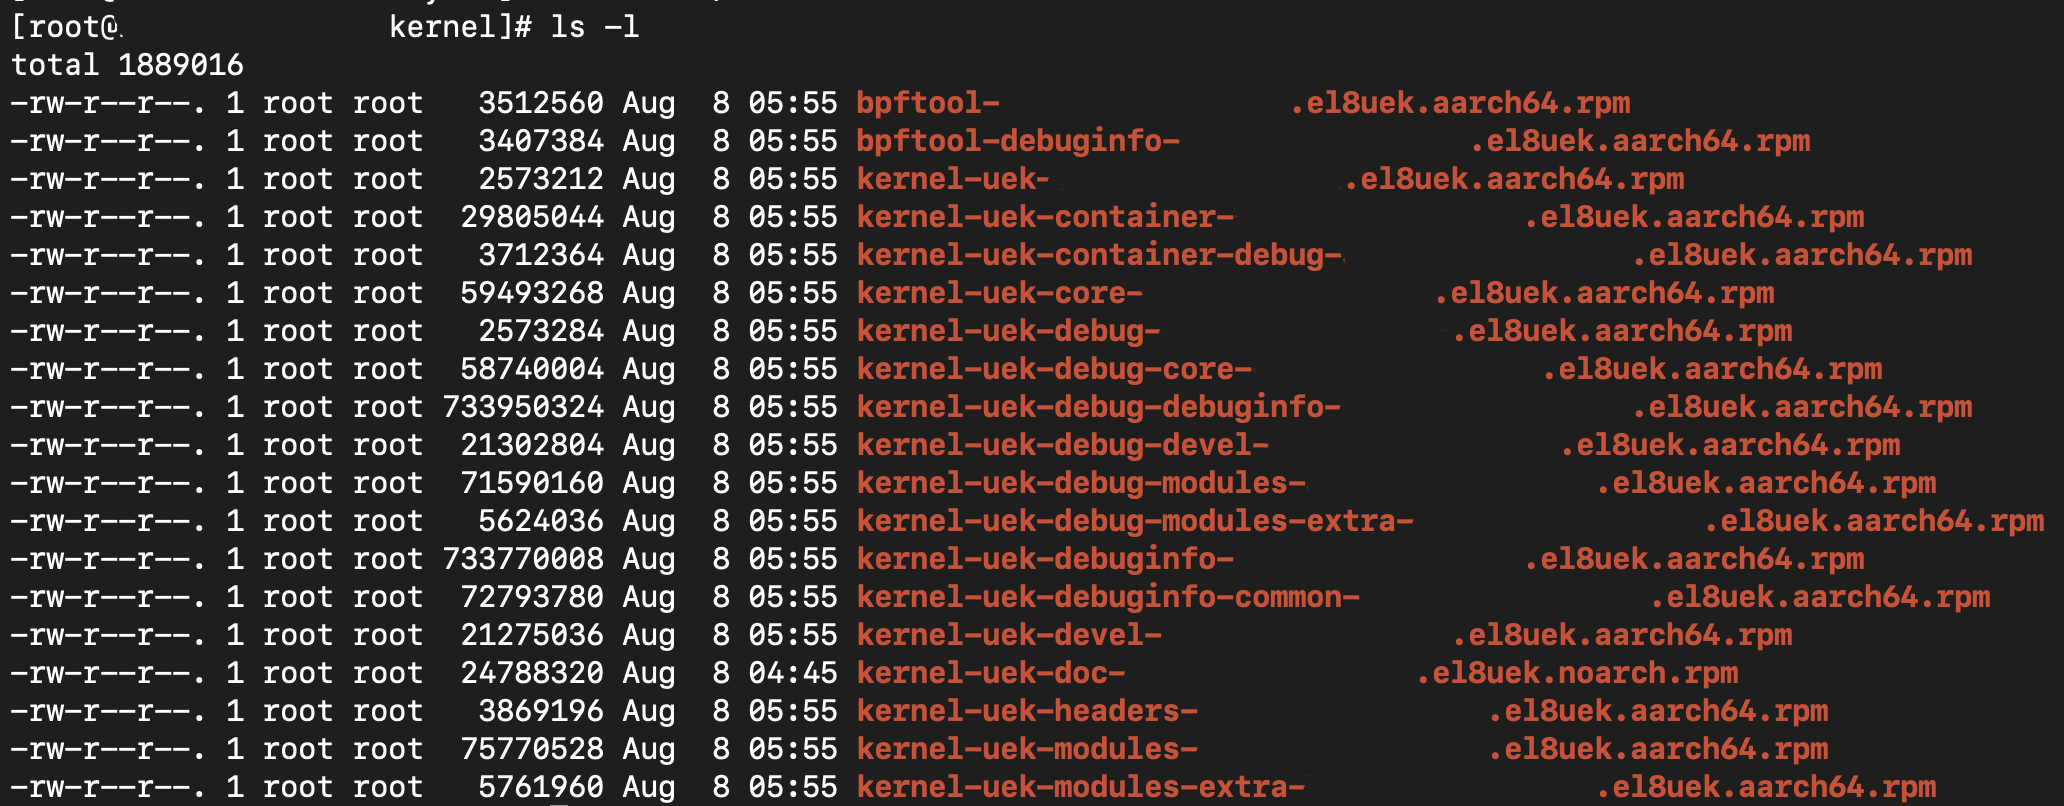
\includegraphics[width=\textwidth]{Images/kernel-rpm.png}
    \captionof{figure}{Kernel RPM Files Downloaded}
    \label{fig:casa}
\end{center}

Once the RPM files were downloaded, the kernel was installed on the host system, as illustrated below:

\begin{center}
    \centering
    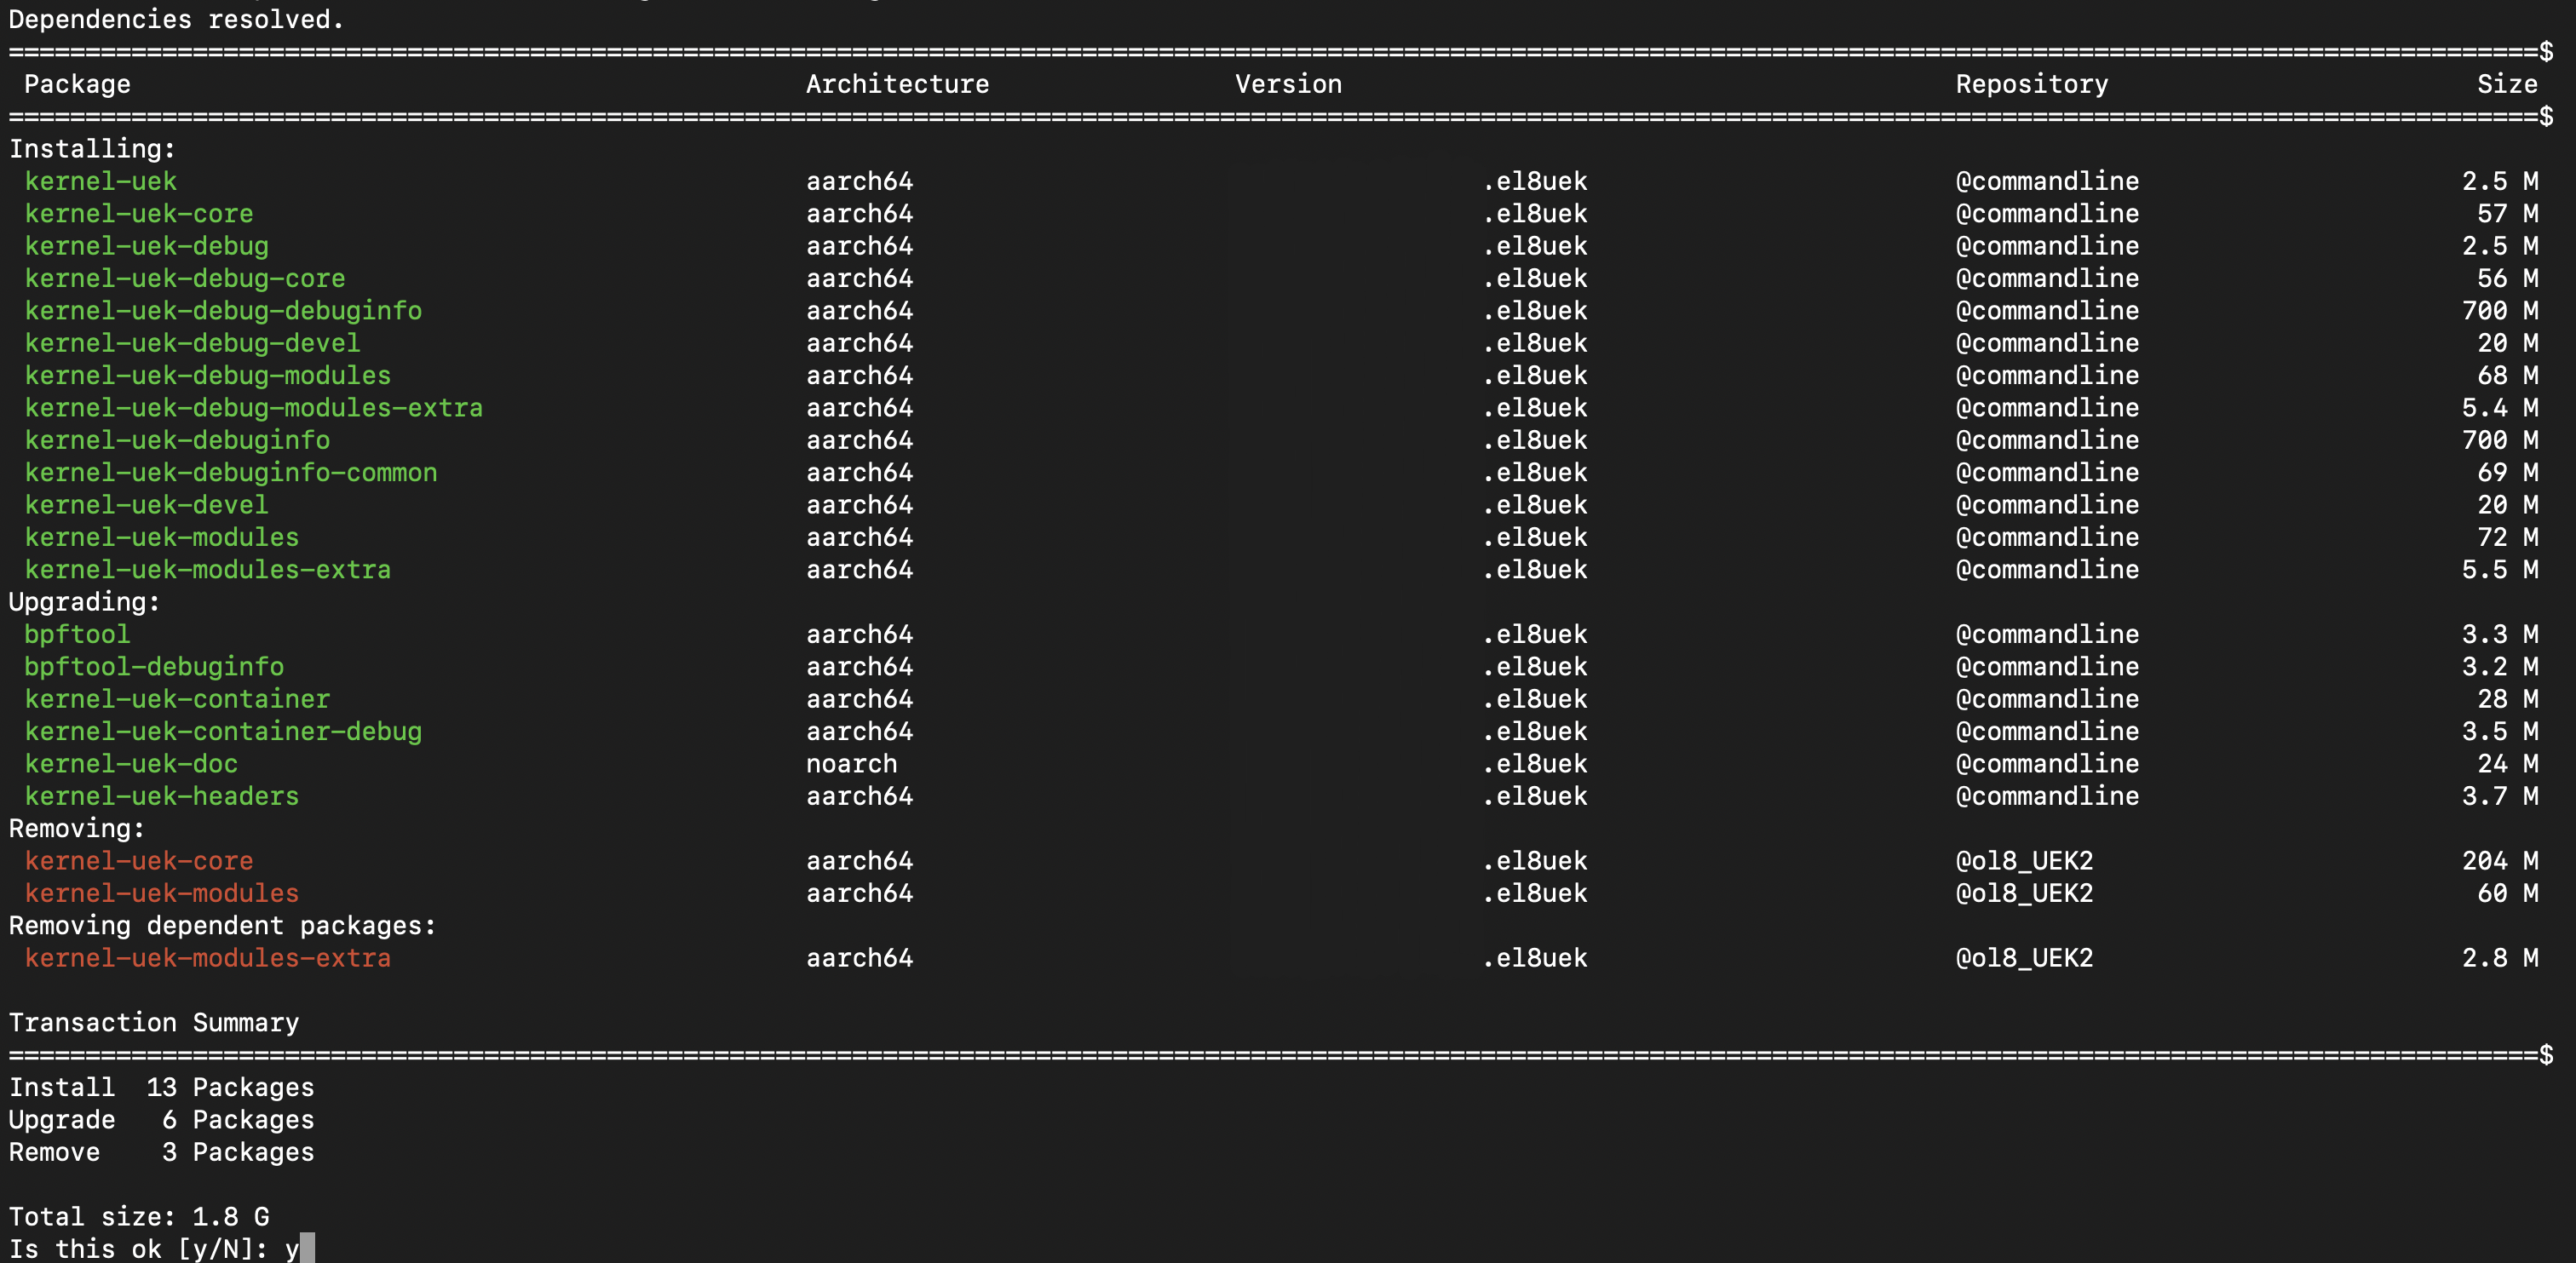
\includegraphics[width=\textwidth]{Images/Kernel-Installation.png}
    \captionof{figure}{Kernel Installation Process}
    \label{fig:casa}
\end{center}

After installation, the host system was rebooted to apply the new kernel. Post-reboot, the correct kernel version was verified using commands such as \texttt{grubby} or \texttt{uname} to confirm that the system was running the desired kernel.

\begin{center}
    \centering
    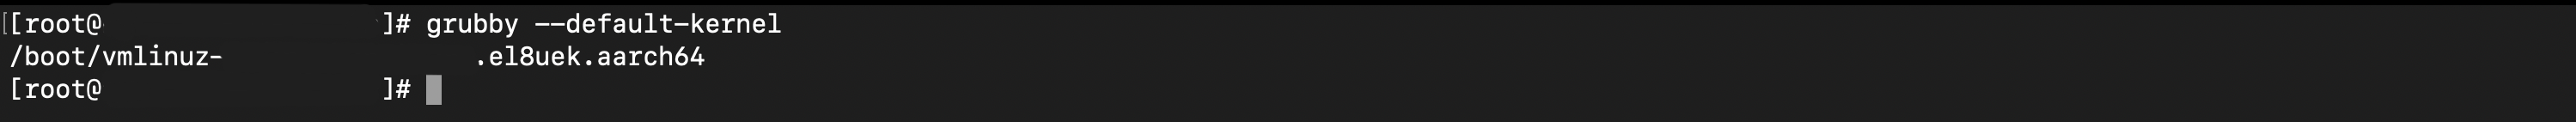
\includegraphics[width=\textwidth]{Images/Kernel-Version.png}
    \captionof{figure}{Verifying the Kernel Version}
    \label{fig:casa}
\end{center}

%% Installation of QEMU and Libvirt
\subsection{Installation of QEMU and Libvirt}

The subsequent step involved the installation of the required versions of QEMU and Libvirt. For tickets focused exclusively on QEMU, only QEMU was installed. However, for tests involving Libvirt, both QEMU and Libvirt needed to be installed to meet the test requirements.\mynewline

To begin with, the repository link for QEMU was assigned to a variable named \texttt{Link}, after which the installation was executed using the \texttt{yum install} command, as shown below:

\begin{center}
    \centering
    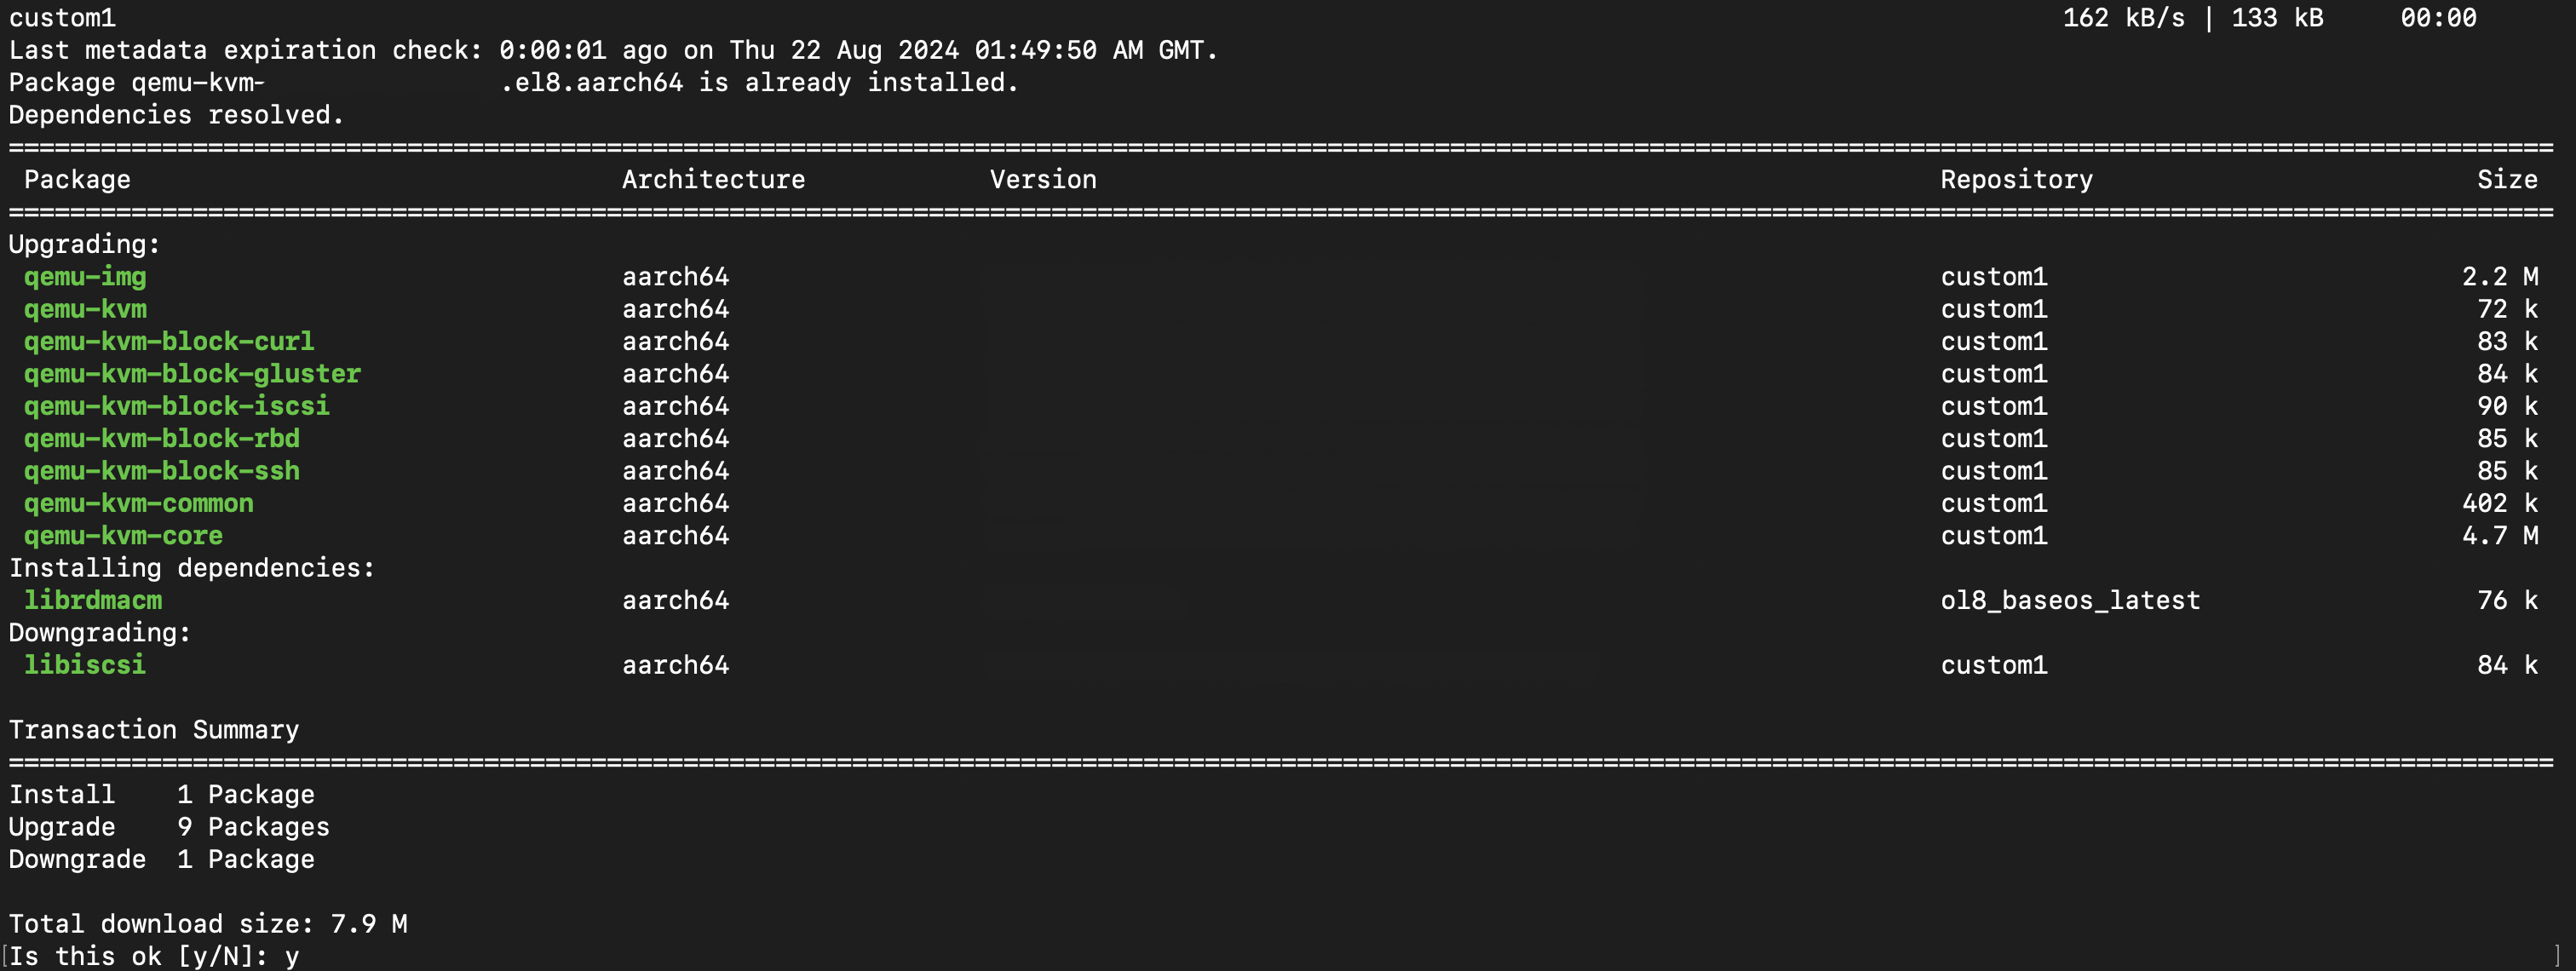
\includegraphics[width=\textwidth]{Images/QEMU-Installation.png}
    \captionof{figure}{QEMU Installation Process}
    \label{fig:casa}
\end{center}

A similar process was followed for installing Libvirt:

\begin{center}
    \centering
    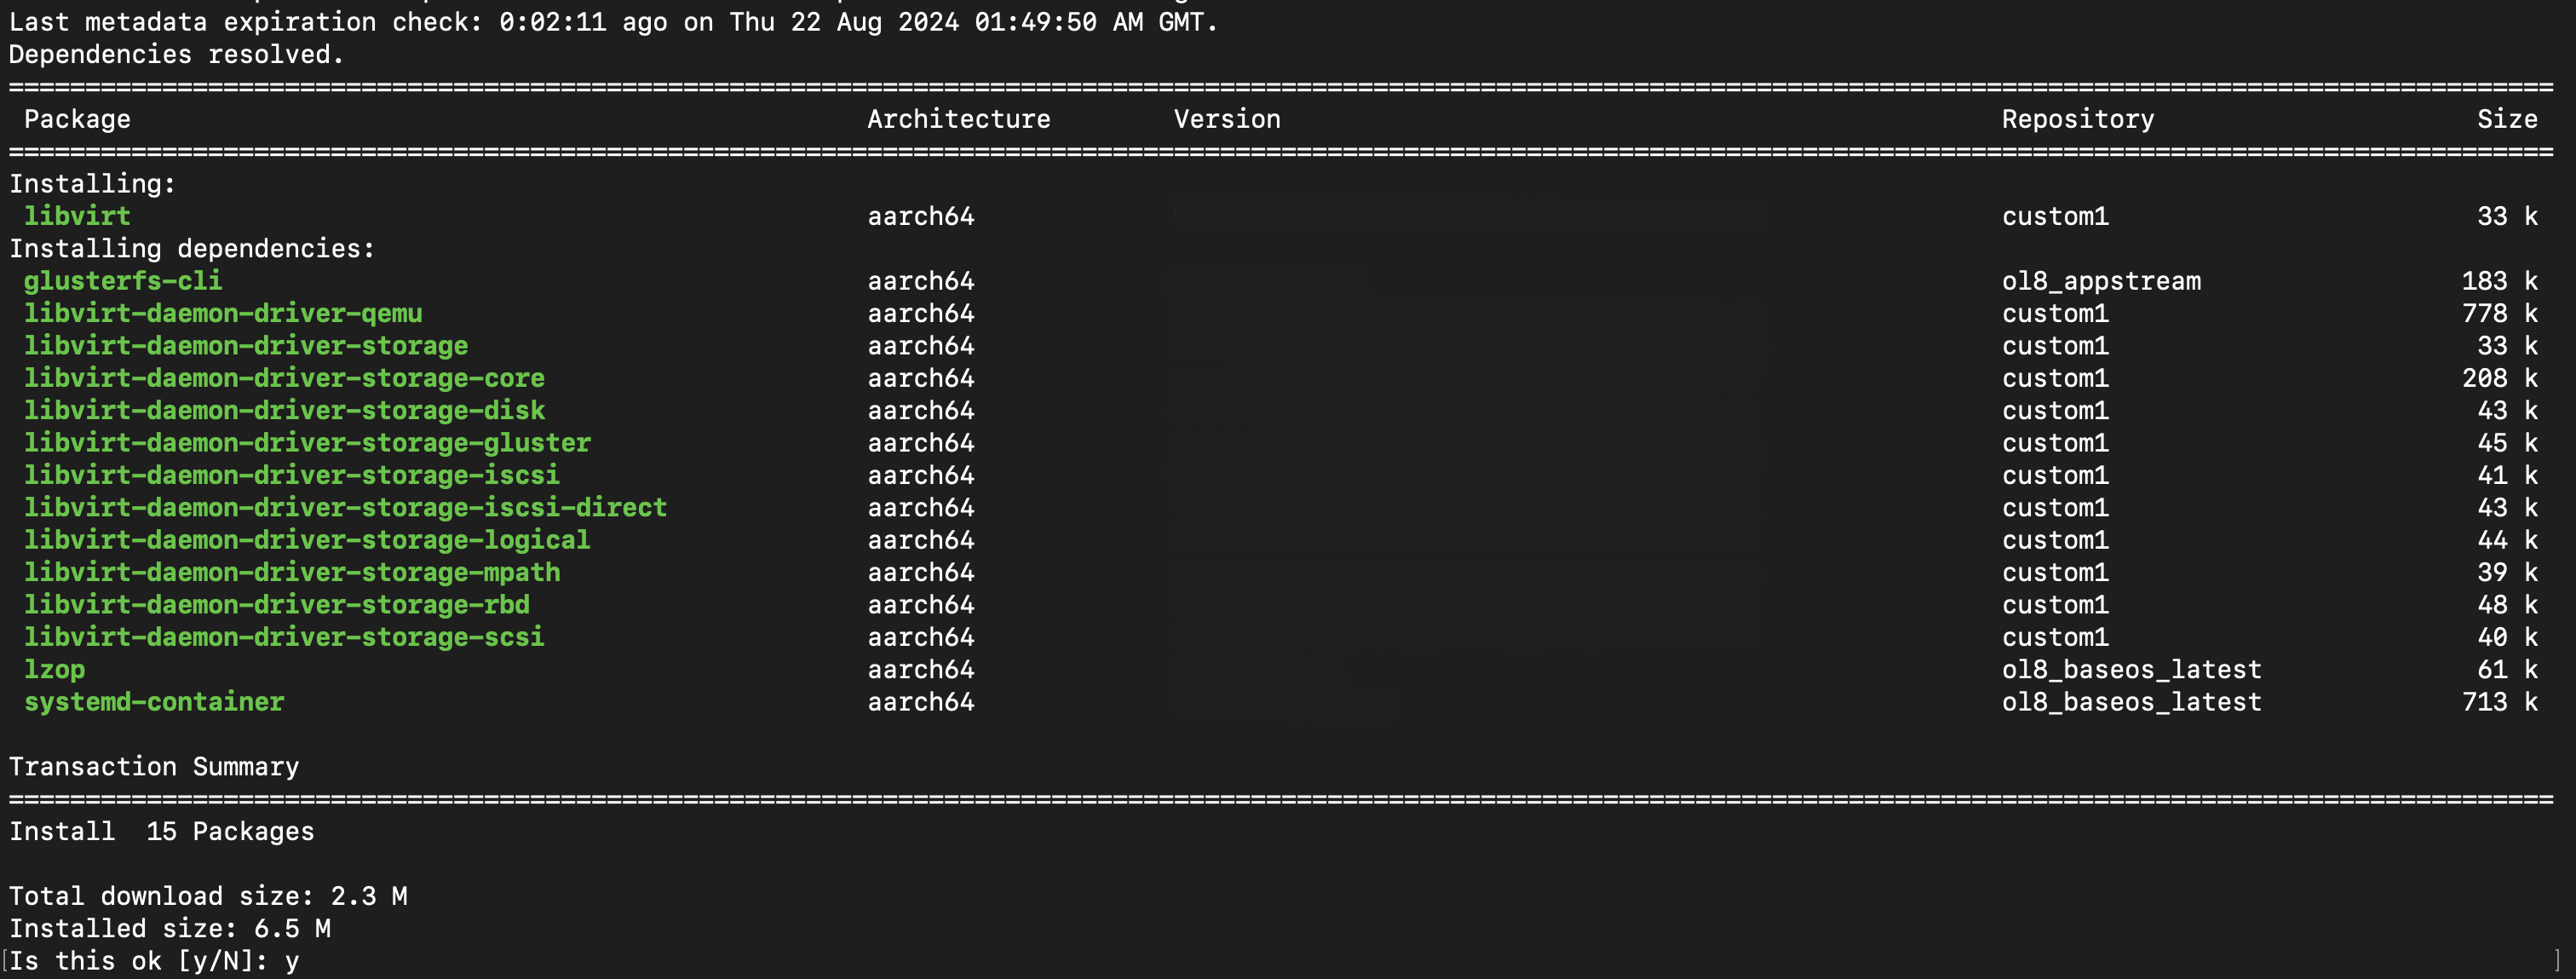
\includegraphics[width=\textwidth]{Images/Libvirt-Installation.png}
    \captionof{figure}{Libvirt Installation Process}
    \label{fig:casa}
\end{center}

After both installations were completed, the versions of QEMU and Libvirt on the host were verified to ensure the correct versions were in place:

\begin{center}
    \centering
    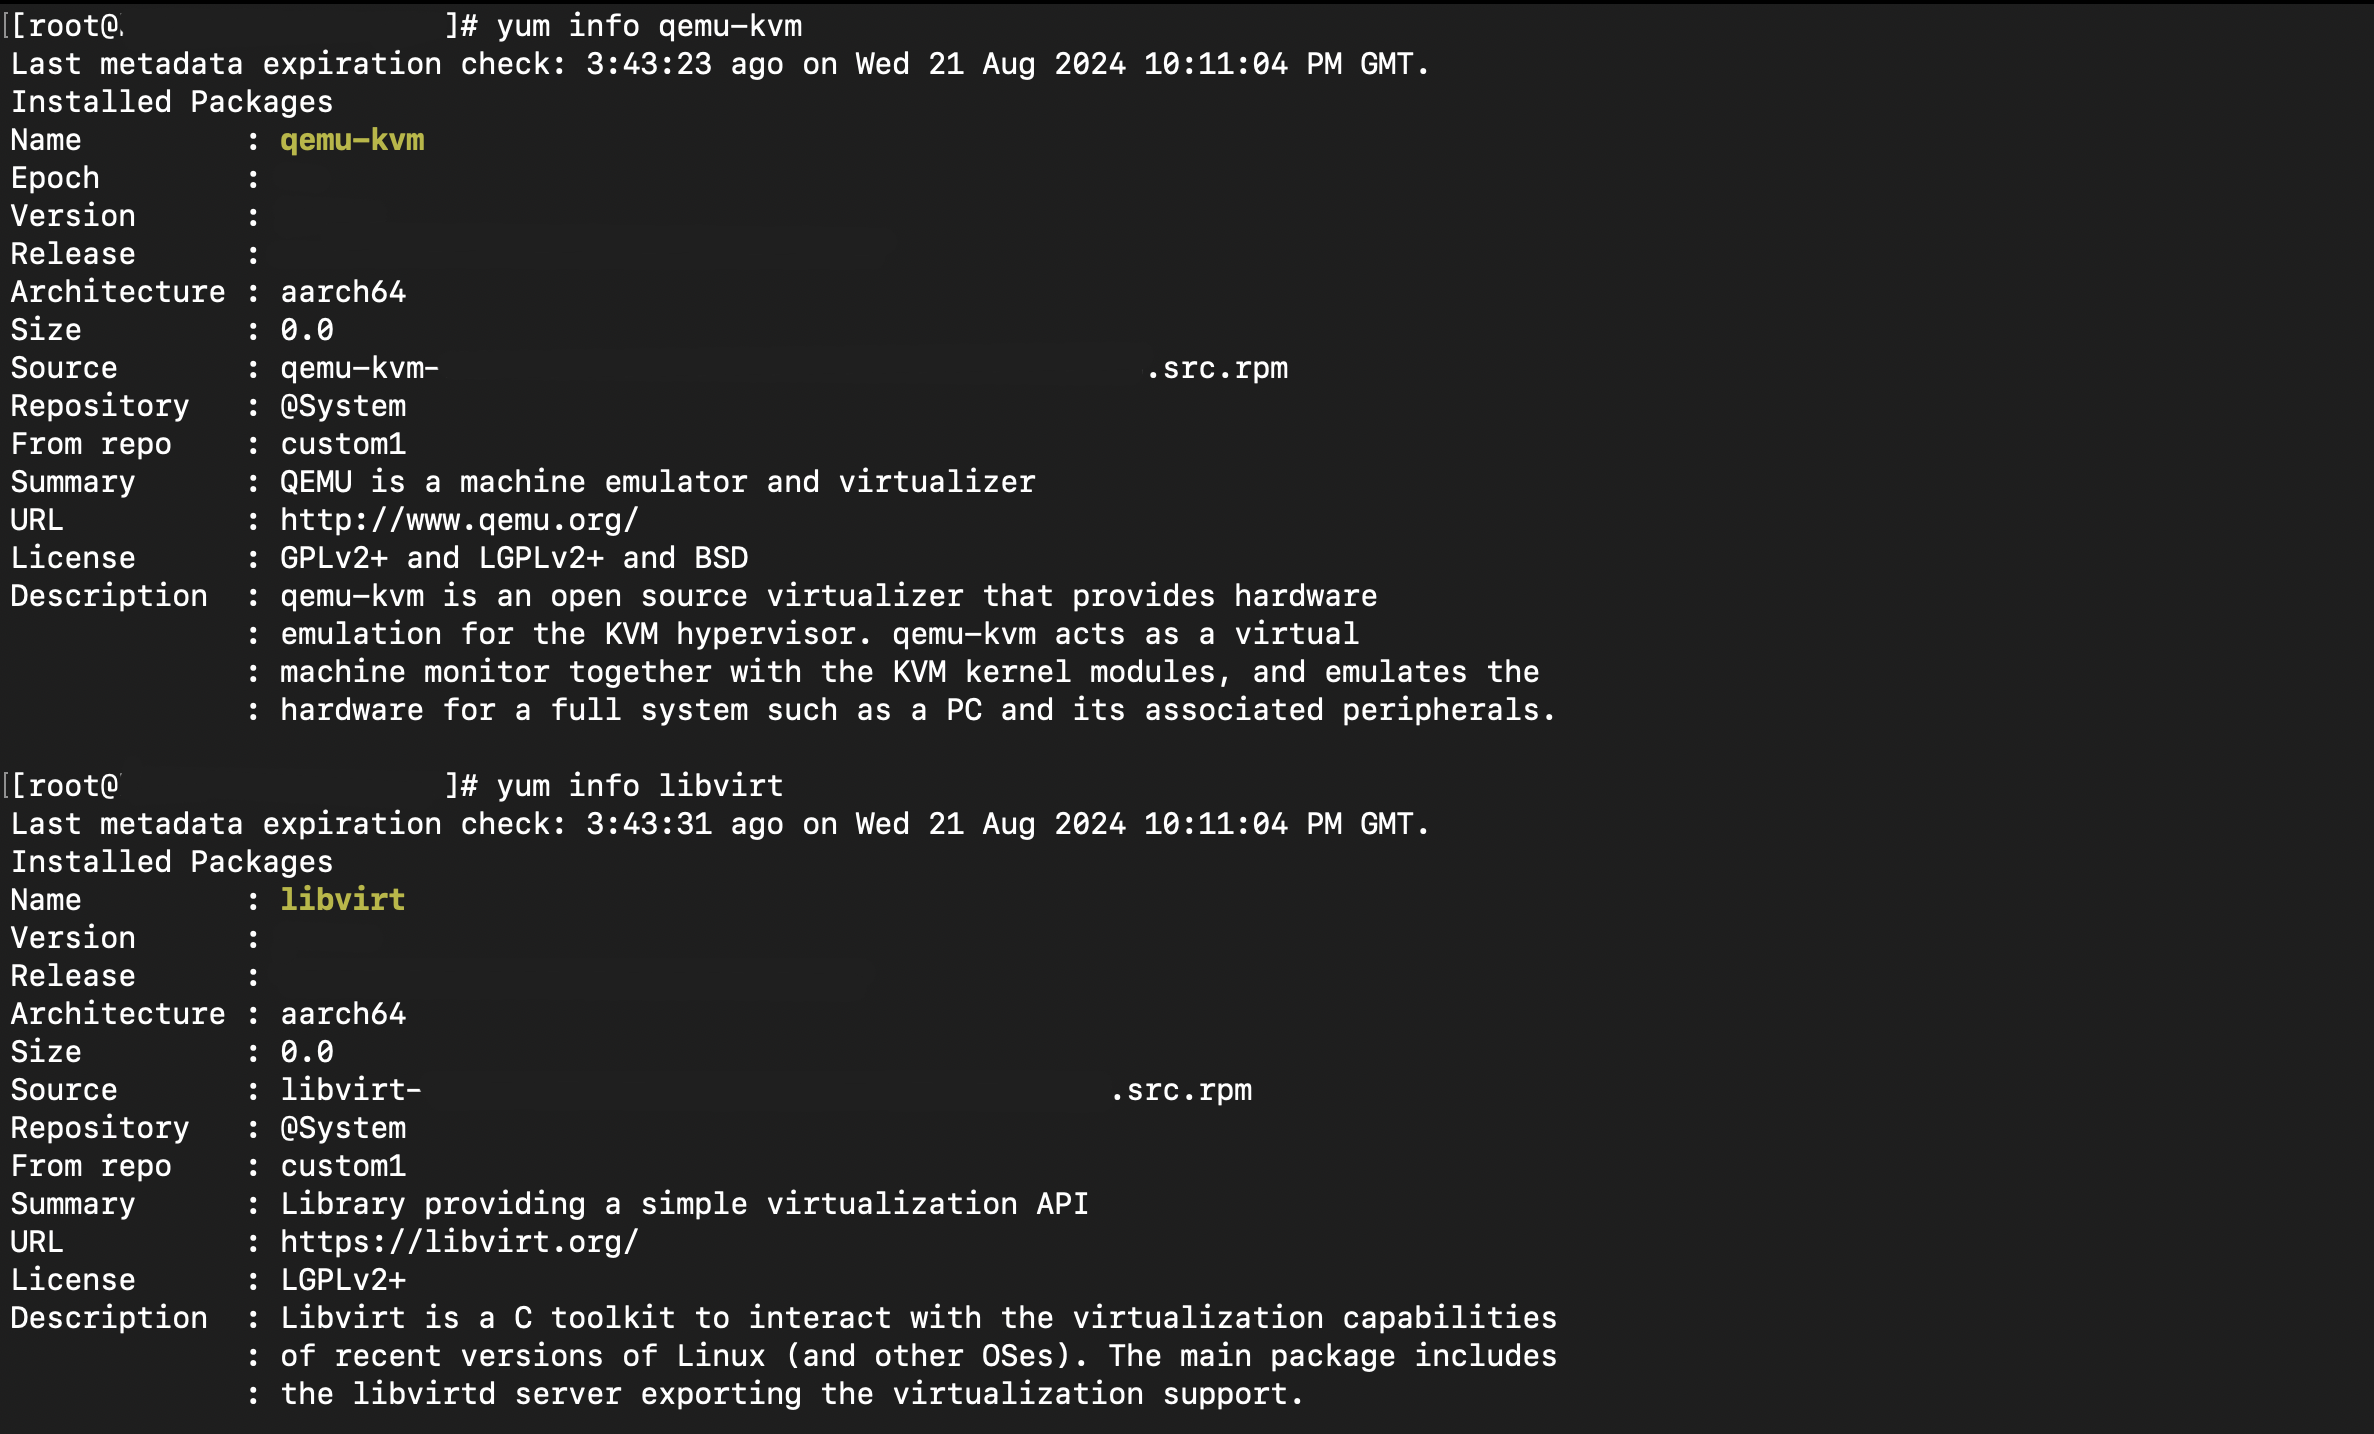
\includegraphics[width=\textwidth]{Images/QEMU & Libvirt Version.png}
    \captionof{figure}{Verification of QEMU and Libvirt Versions}
    \label{fig:casa}
\end{center}


%% OVMF/AAVMF
\subsection{OVMF/AAVMF}

To ensure proper virtualization support across different platforms, I verified the presence of essential files for OVMF (used for AMD and Intel hosts) and AAVMF (used for ARM hosts) on the system.\mynewline

Initially, it was observed that the directory \texttt{/usr/share/AAVMF/} contained fewer than the expected number of files, with only six present:

\begin{center}
    \centering
    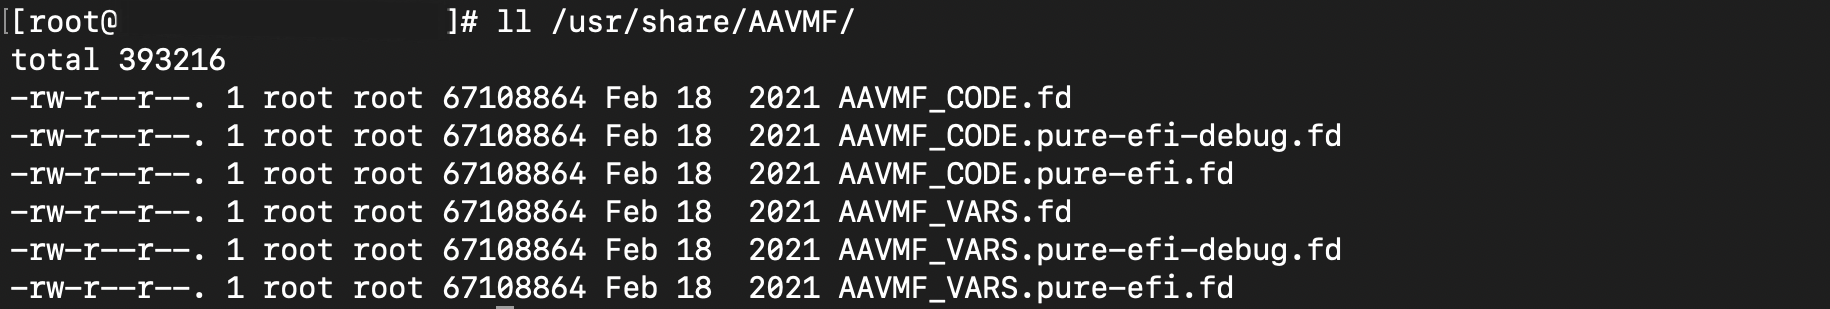
\includegraphics[width=\textwidth]{Images/AAVMF Incomplete Files.png}
    \captionof{figure}{Incomplete AAVMF Files}
    \label{fig:casa}
\end{center}

To address this issue, a new yum repository was created to download the complete set of necessary files. The repository was configured as follows:

\begin{center}
    \centering
    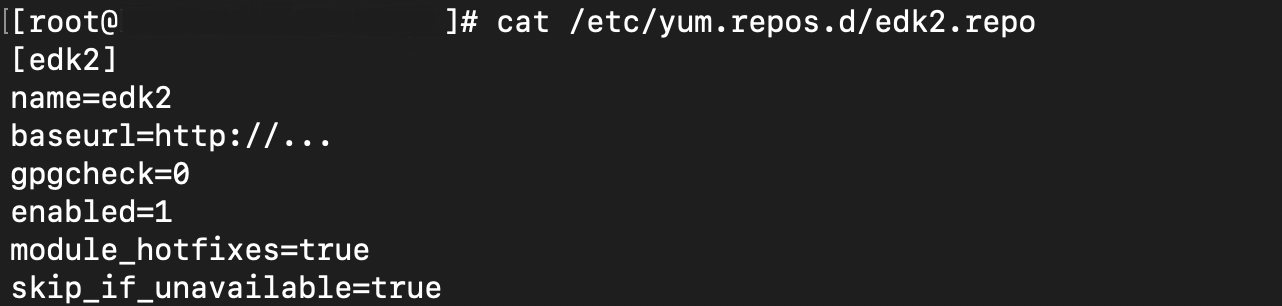
\includegraphics[width=\textwidth]{Images/Edk2 Yum Repository.png}
    \captionof{figure}{edk2 Yum Repository Configuration}
    \label{fig:casa}
\end{center}

The new files were then installed using the following command:

\begin{center}
    \centering
    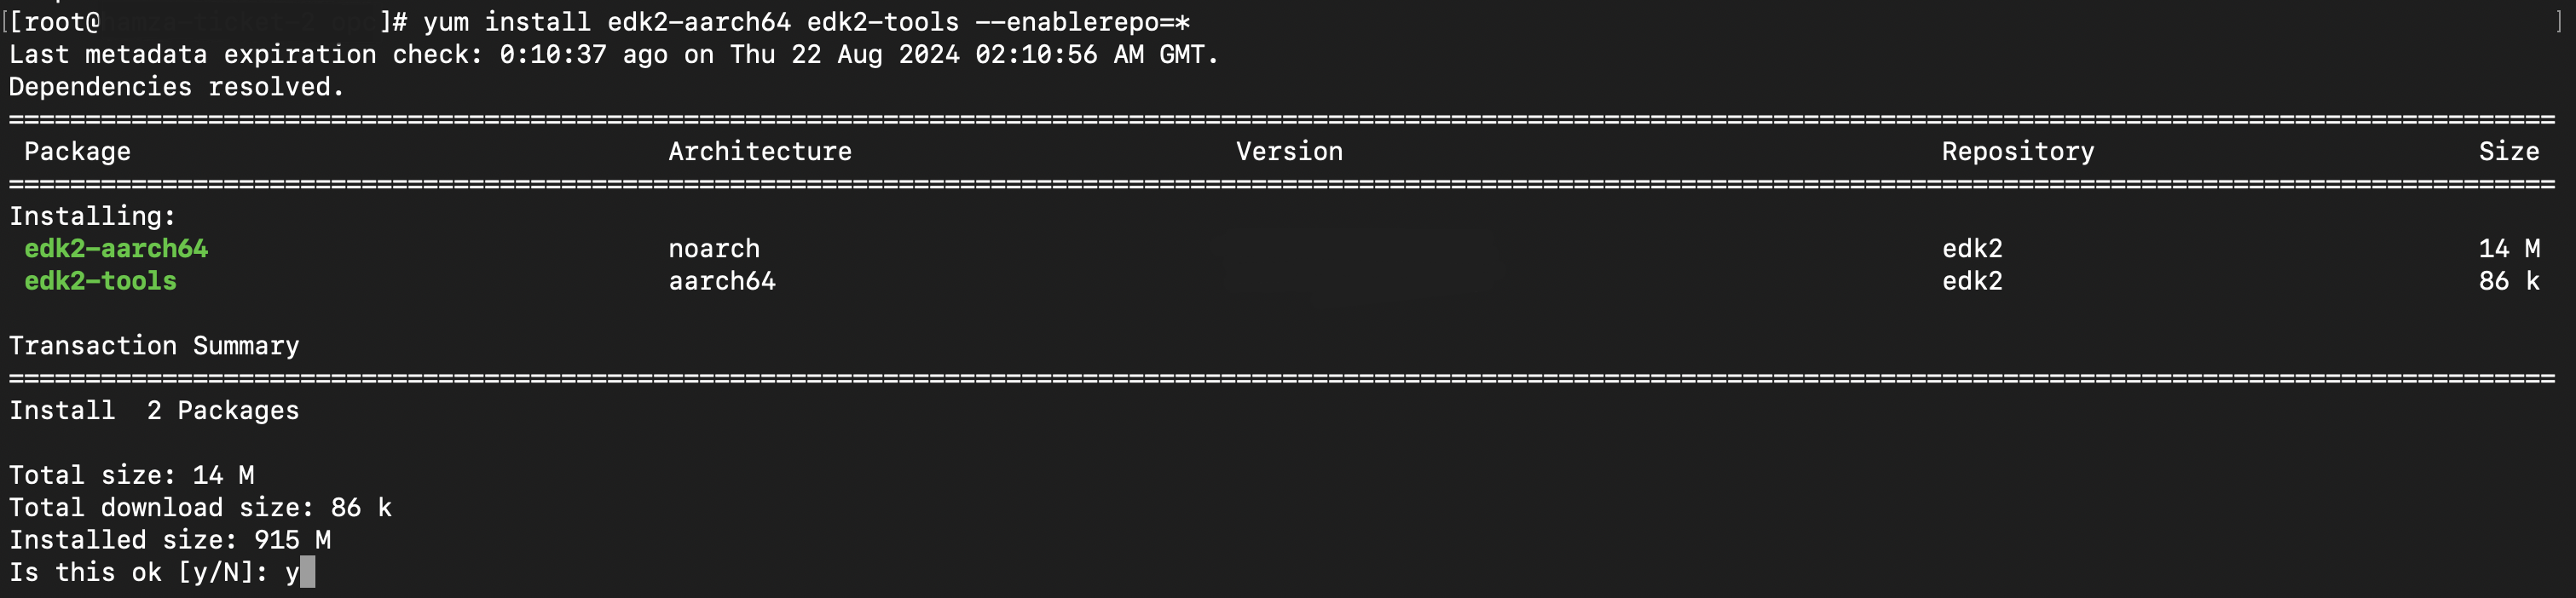
\includegraphics[width=\textwidth]{Images/EDK2 Installation.png}
    \captionof{figure}{Installation of edk2 Files}
    \label{fig:casa}
\end{center}

Finally, the directory \texttt{/usr/share/AAVMF/} was checked again to confirm that all necessary files were now correctly installed:

\begin{center}
    \centering
    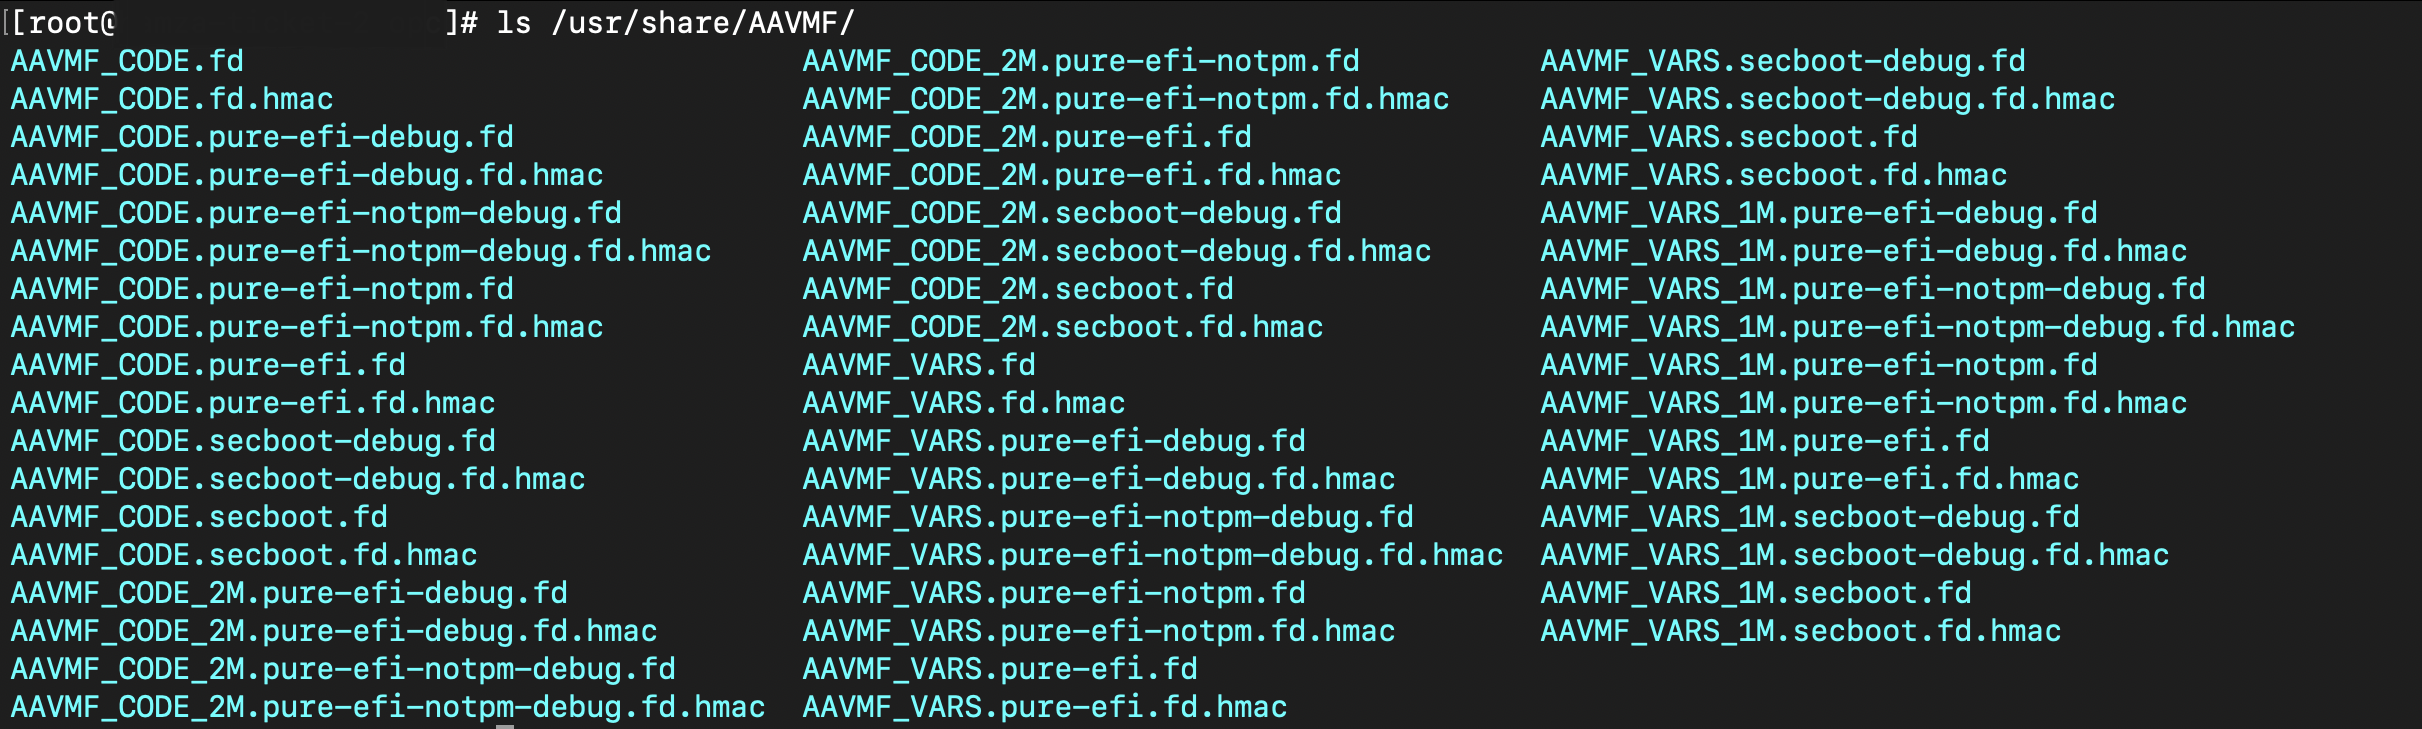
\includegraphics[width=\textwidth]{Images/AAVMF Files.png}
    \captionof{figure}{Verified AAVMF Files}
    \label{fig:casa}
\end{center}

%% ISO Installation and Image Creation
\subsection{ISO Installation and Image Creation}

With the environment prepared, the next step involved downloading and installing the ISO files necessary for the guest OSs. These included ISOs for Oracle Linux 7.9, 8.9 and 8.10.\mynewline

Creating the disk image was a critical process in both QEMU and Libvirt tests. A disk image is essentially a file that contains the complete contents and structure of a storage device, such as a hard drive. This image is used by virtual machines to simulate the presence of an actual physical disk, allowing the guest OS to function as if it were running on its own dedicated hardware.\mynewline

For QEMU, the image was created using the following command:

\begin{center}
    \centering
    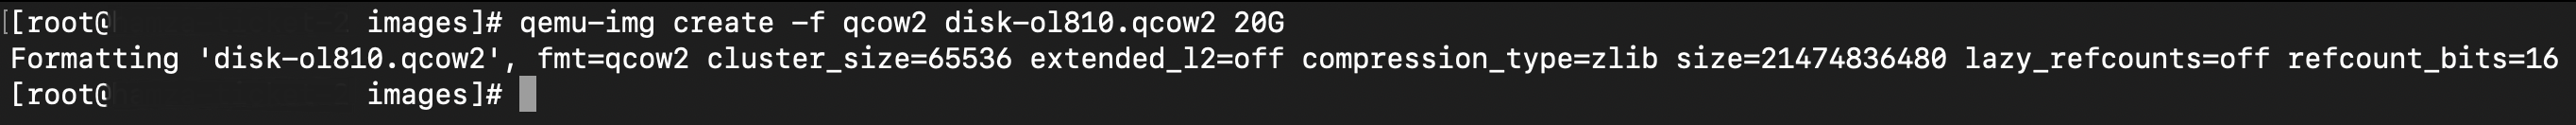
\includegraphics[width=\textwidth]{Images/Disk Image Creation QEMU.png}
    \captionof{figure}{Creating Disk Image Using QEMU}
    \label{fig:casa}
\end{center}

In this case, the image format chosen was QCOW2 instead of RAW. The QCOW2 format offers several advantages, including the ability to take snapshots and compress the image to save space, which is especially useful in test environments where flexibility and storage efficiency are important. The RAW format, on the other hand, provides better performance but at the cost of increased storage space and fewer features, making QCOW2 the preferred choice for this project.\mynewline

When using Libvirt, the process involves some additional steps. First, the Libvirt daemon must be started to manage the virtualization services:

\begin{center}
    \centering
    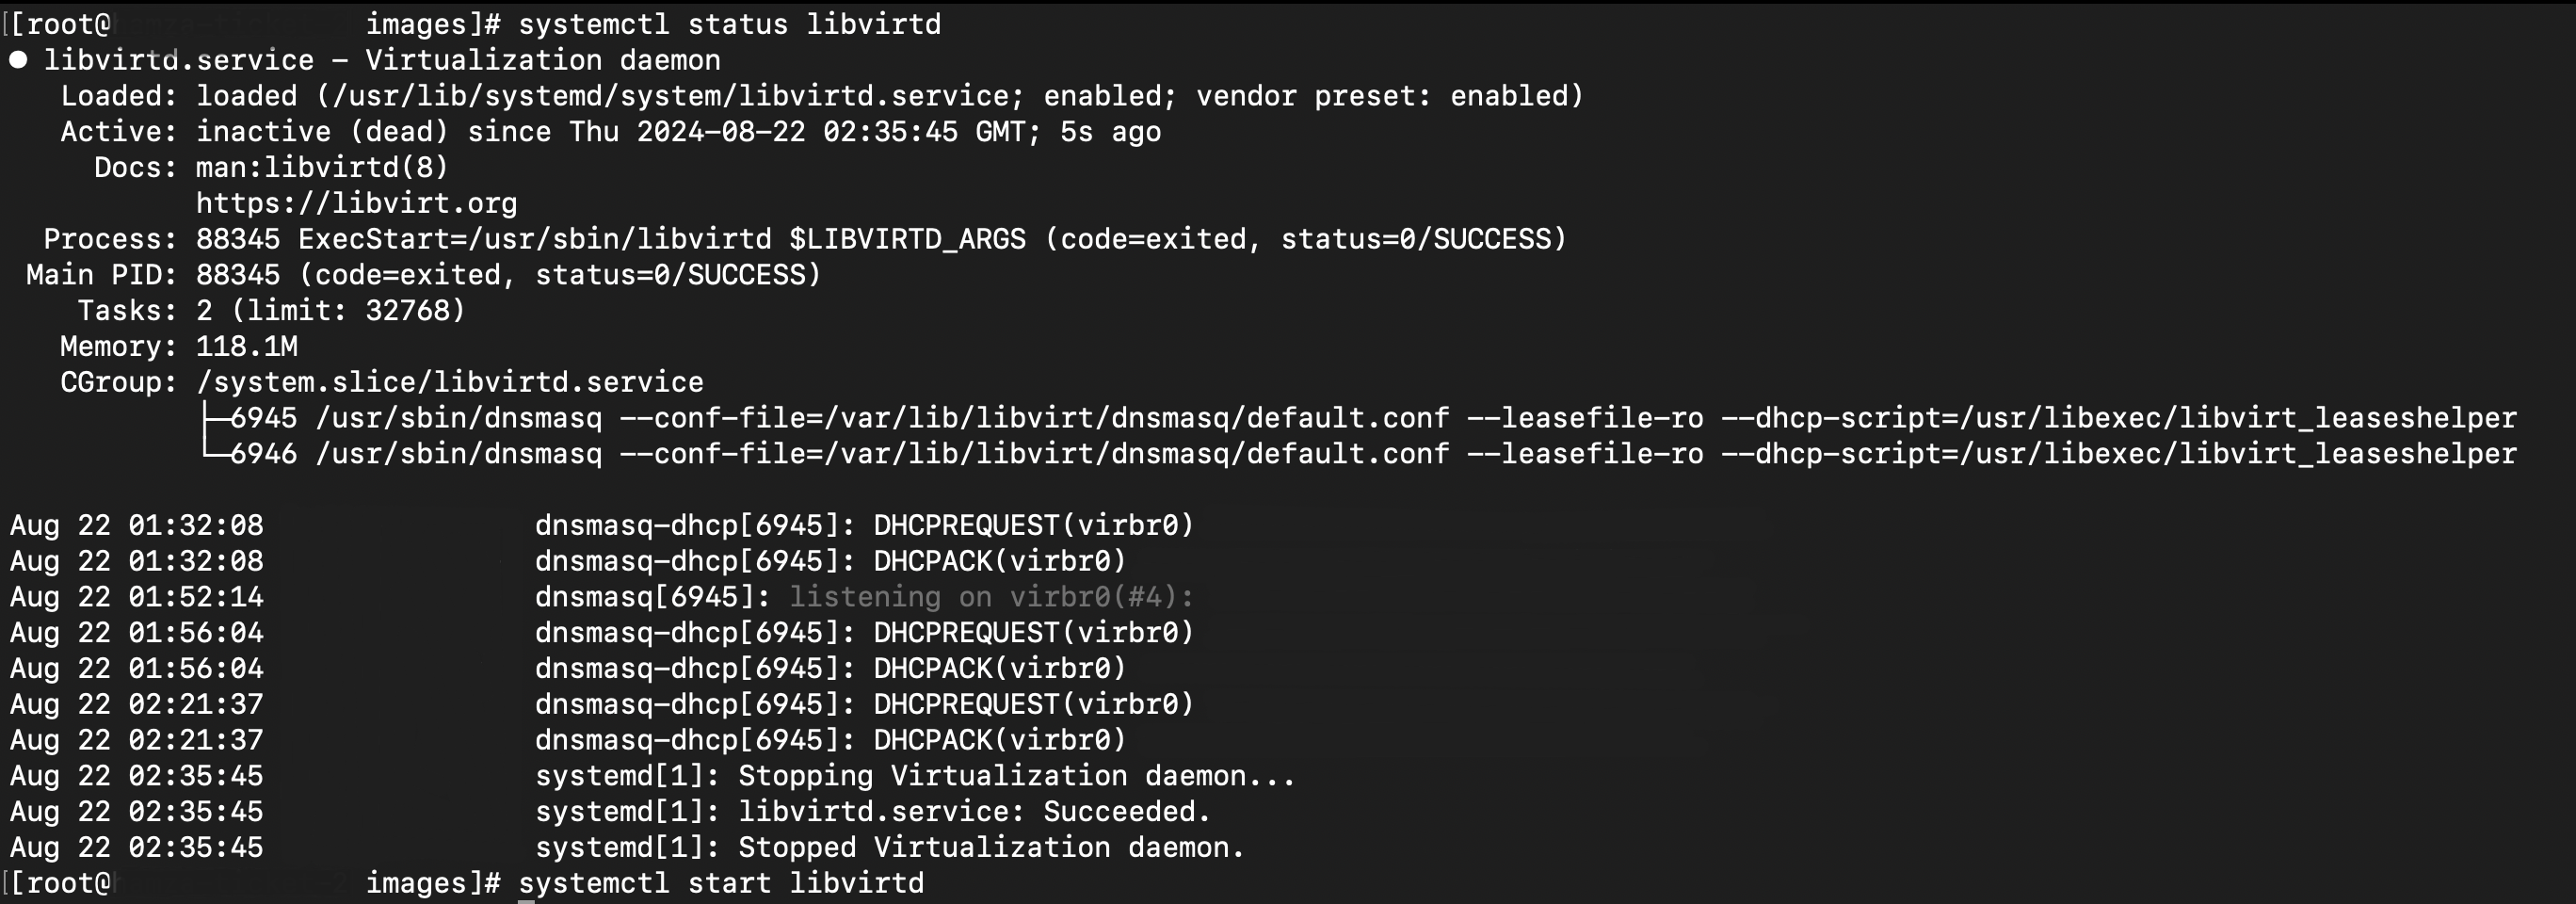
\includegraphics[width=\textwidth]{Images/Starting Libvirtd.png}
    \captionof{figure}{Starting Libvirt Daemon}
    \label{fig:casa}
\end{center}

Next, a storage pool needs to be created. A storage pool is a collection of storage volumes managed by Libvirt, where virtual machines can store their disk images. It acts as an abstraction layer, allowing easy management of storage resources for virtual environments. After creating the storage pool, it is started to make it available for use:

\begin{center}
    \centering
    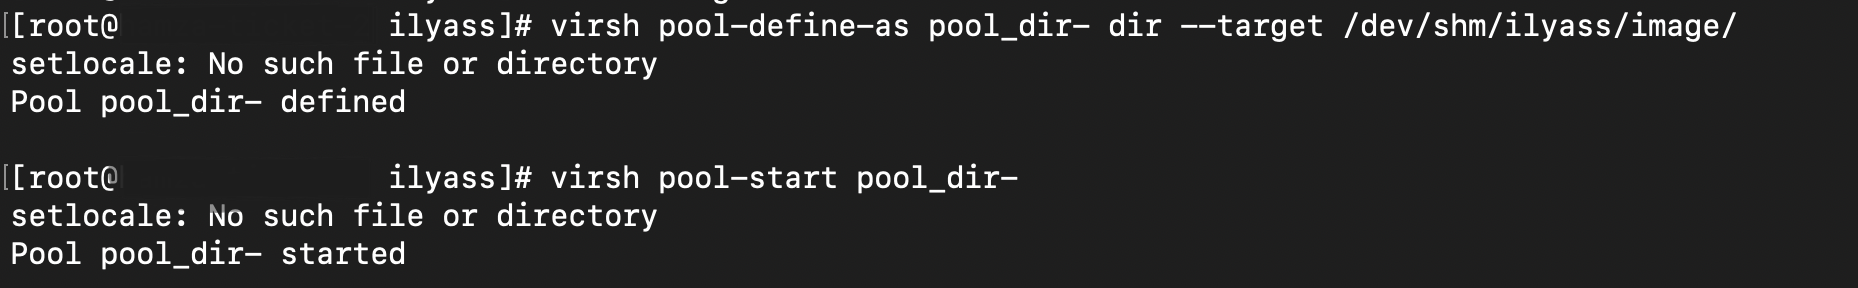
\includegraphics[width=\textwidth]{Images/Storage pool creation.png}
    \captionof{figure}{Creating and Starting the Storage Pool}
    \label{fig:casa}
\end{center}

Finally, the required disk image is created within this storage pool:

\begin{center}
    \centering
    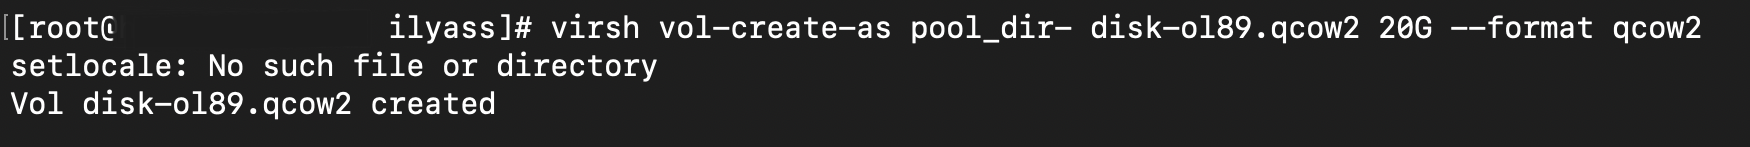
\includegraphics[width=\textwidth]{Images/Disk Image Creation Libvirt.png}
    \captionof{figure}{Creating Disk Image Using Libvirt}
    \label{fig:casa}
\end{center}

%% Creating the VM Using QEMU
\subsection{Creating the VM Using QEMU}

For QEMU-based tests, the virtual machine (VM) was created using a detailed command that specified the necessary parameters, including CPU type, memory allocation, and the disk image. This command enabled the configuration and launch of the VM, ensuring it was tailored to meet the test requirements.\mynewline

The command used to create and run the VM is shown below:

\begin{center}
    \centering
    \includegraphics[width=\textwidth]{Images/VM Creation with QEMU.png}
    \captionof{figure}{Creating VM Using QEMU}
    \label{fig}
\end{center}

This command includes several important components:

\begin{itemize}
    \item \textbf{-boot d}: This option tells QEMU to boot from the first virtual CD-ROM drive;
    \item \textbf{-machine virt,accel=kvm,gic-version=3}: Specifies the machine type and enables KVM acceleration, which improves performance by allowing the VM to run directly on the host's hardware;
    \item \textbf{-m 32G,slots=6,maxmem=64G}: Allocates 32GB of memory to the VM with six additional memory slots, allowing the memory to be expanded up to 64GB;
    \item \textbf{-cpu host,+host-phys-bits}: This option uses the host CPU model and enables the use of physical address bits, which can improve performance by allowing the VM to use more memory addresses;
    \item \textbf{-smp cpus=32,cores=32,threads=2,sockets=1,maxcpus=64}: Configures the VM to use 32 CPUs, organized into 32 cores with 2 threads per core, and allows the number of CPUs to scale up to 64;
    \item \textbf{-drive file=/dev/shm/ilyass/image/disk-ol89.qcow2}: Specifies the QCOW2 disk image for the VM;
    \item \textbf{-drive file=/usr/share/AAVMF/AAVMF\_CODE.pure-efi.fd,if=pflash,format\\=raw,unit=0,readonly=on}: Loads the UEFI firmware code for the VM, allowing it to boot using UEFI;
    \item \textbf{-drive file=/tmp/AAVMF\_VARS.pure-efi.fd,if=pflash,format=raw,unit=1:\\} Specifies the UEFI variables file, which stores information like boot order and settings;
    \item \textbf{-device pcie-root-port,io-reserve=0,pref64-reserve=32M,port=2,chassis=2,id\\=pciroot2,bus=pcie.0,addr=0x2}: Adds a PCIe root port to the VM, which is essential for hot-plugging devices like VNICs;
    \item \textbf{-chardev socket,id=mon\_vm,path=/tmp/hmp\_vm1,server=on,wait=off:\\} Configures a character device for QEMU’s monitor interface, allowing real-time management of the VM;
    \item \textbf{-mon chardev=mon\_vm,mode=readline}: Sets up the monitor interface for interactive commands;
    \item \textbf{-qmp unix:/tmp/qmp\_vm1,server=on,wait=off}: Enables QEMU’s QMP (QEMU Machine Protocol) server, providing a powerful API for VM management;
    \item \textbf{-nodefaults}: Disables QEMU’s default devices, giving full control over the VM’s configuration;
    \item \textbf{-vnc :2 -vga std}: Enables VNC (Virtual Network Computing) for remote access to the VM’s display and sets up a standard VGA display;
    \item \textbf{-netdev user,id=netdev1,hostfwd=tcp::6002-:22}: Configures user-mode networking with port forwarding, allowing SSH access to the VM on port 6002;
    \item \textbf{-device virtio-net-pci,id=net1,netdev=netdev}: Adds a virtualized network interface to the VM, connecting it to the user-mode network.
\end{itemize}

This setup ensures that the VM is fully optimized for performance and scalability, making it suitable for the rigorous testing scenarios.

%% Creating VM Using Libvirt
\subsection{Creating the VM Using Libvirt}

In the Libvirt-based tests, the virtual machine (VM) creation was handled through Libvirt commands, providing a streamlined approach for managing VM configurations, storage pools, and other settings. This method offers fine-grained control over the VM setup and facilitates the use of advanced features provided by Libvirt.\mynewline

The command used to create the VM is illustrated in the image below:

\begin{center}
    \centering
    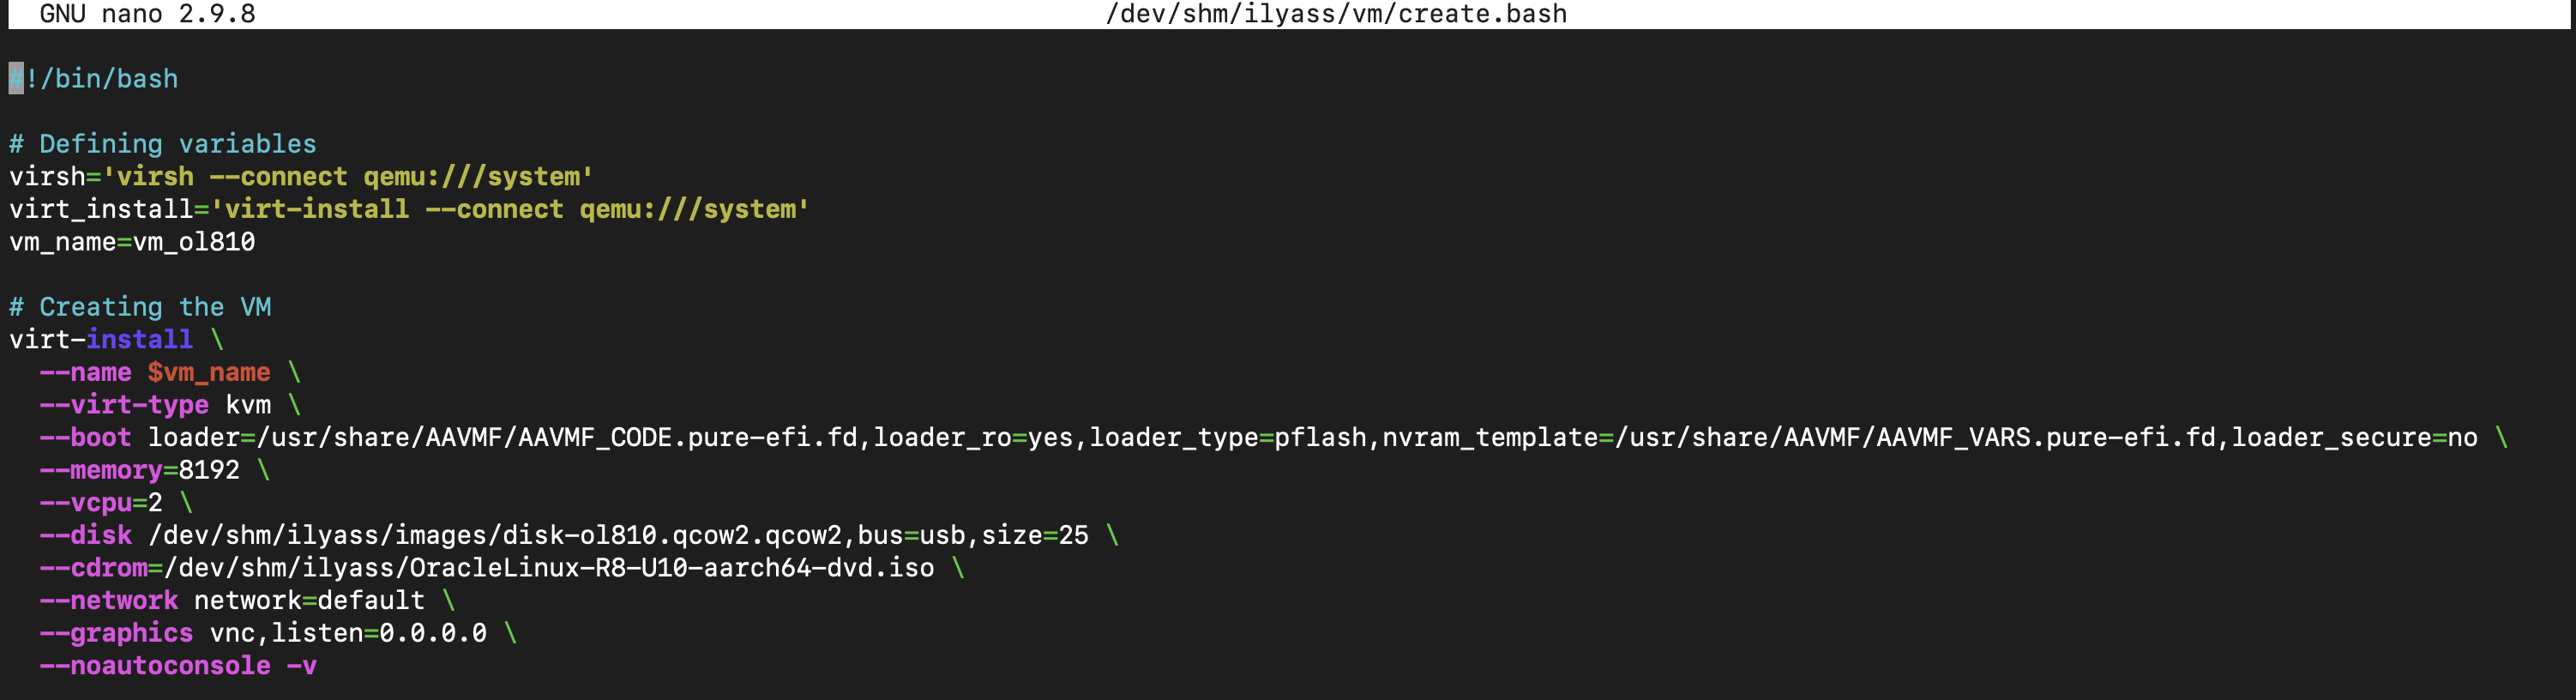
\includegraphics[width=\textwidth]{Images/VM Cration Using Libvirt.png}
    \captionof{figure}{Creating VM Using Libvirt}
    \label{fig}
\end{center}

The command includes several key elements:

\begin{itemize}
    \item \textbf{virsh='virsh --connect qemu:///system'}: Sets up the \texttt{virsh} command to interact with the QEMU system through Libvirt;
    \item \textbf{virt\_install='virt-install --connect qemu:///system'}: Defines the \texttt{virt-install} command for creating and installing the VM;
    \item \textbf{vm\_name=vm\_ol810}: Specifies the name of the VM as 'vm\_ol810';
    \item \textbf{--virt-type kvm}: Specifies that the VM will use KVM as the virtualization type;
    \item \textbf{--boot loader=...}: Configures the boot loader with UEFI firmware, including the secure boot options and NVRAM template;
    \item \textbf{--network network=default}: Connects the VM to the default virtual network;
    \item \textbf{--graphics vnc,listen=0.0.0.0}: Configures VNC for remote graphical access to the VM;
    \item \textbf{--noautoconsole -v}: Prevents automatic console connection and enables verbose output for better logging.
\end{itemize}

This setup provides a comprehensive approach to VM creation using Libvirt, ensuring proper configuration and access for subsequent testing and management.

%% Interaction with the VM
\subsection{Interaction with the VM}

Interacting with a virtual machine (VM) is a crucial aspect of managing and utilizing virtualized environments. Various methods can be employed to access and control the VM, each offering different functionalities and levels of control. Below, we explore two primary methods: using VNC for graphical access and leveraging the QEMU Monitor for advanced management.

%% Using VNC
\subsubsection[Using VNC]{Using VNC}

Virtual Network Computing (VNC) is a widely-used protocol for remote graphical access to a VM. By connecting through VNC, users can interact with the VM's desktop environment as if they were physically present at the machine. This approach is especially beneficial for:

\begin{itemize}
    \item \textbf{Visual Interaction}: VNC allows for direct interaction with the VM's graphical user interface (GUI), making it easier to perform visual checks, configure settings, and troubleshoot issues from a remote location;
    \item \textbf{Basic Operations}: For tasks that require GUI interaction, such as software installations or configuration changes that are more intuitive with a graphical interface, VNC provides an effective solution;
    \item \textbf{Remote Access}: VNC facilitates remote access to the VM, which is advantageous for users who need to work from different locations or for administrators managing multiple VMs.
\end{itemize}

To utilize VNC for interacting with the VM, it is necessary to first configure the VM with a VNC server. Once configured, we can connect to the VM using a VNC client.

\begin{center}
    \centering
    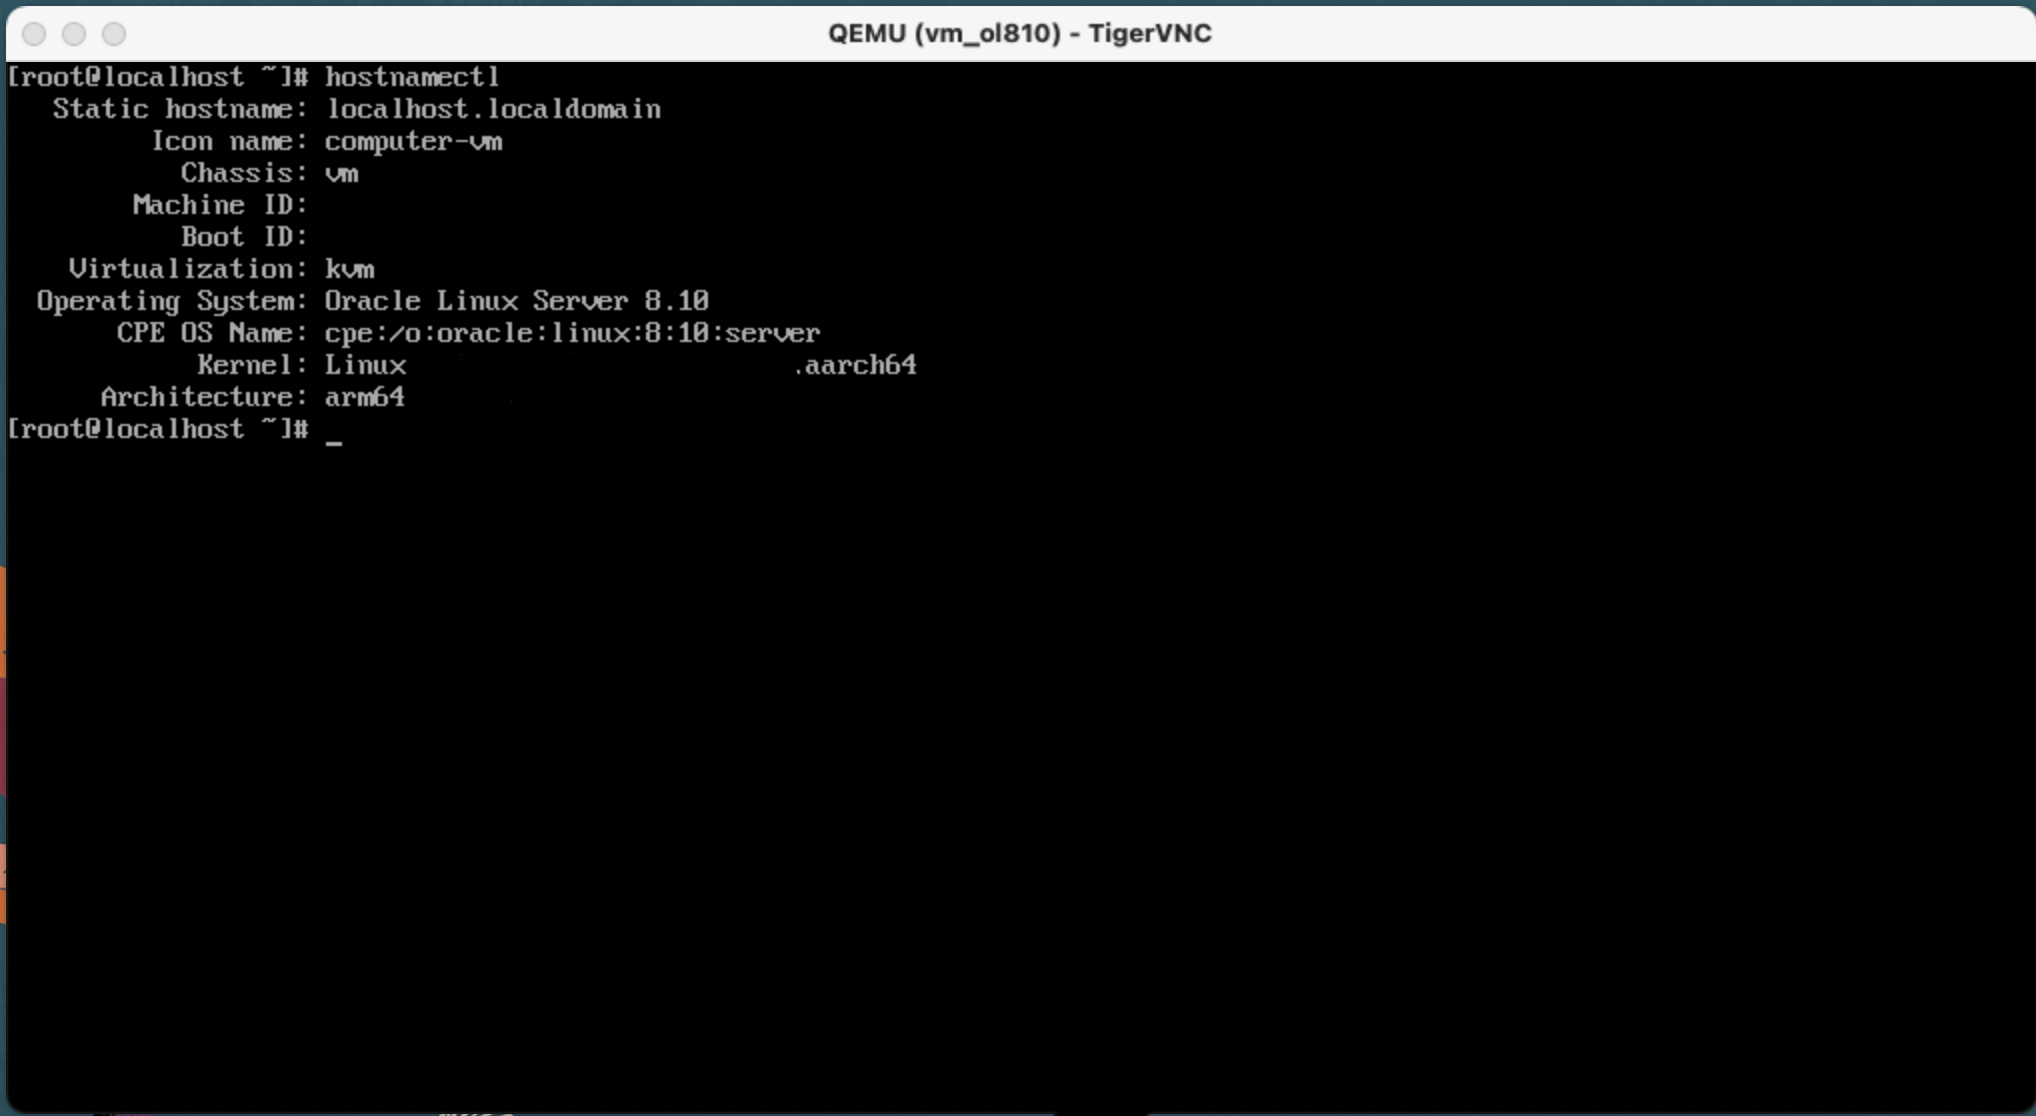
\includegraphics[width=\textwidth]{Images/VNC Client.png}
    \captionof{figure}{VNC Client}
    \label{fig}
\end{center}

%% Using QEMU Monitor
\subsubsection[Using QEMU Monitor]{Using QEMU Monitor}

The QEMU Monitor is a powerful tool that provides a command-line interface for managing and interacting with a VM. It offers several advanced features, making it an essential component for users who need deeper control over the VM's operations. Key functionalities include:

\begin{itemize}
    \item \textbf{Hardware Configuration}: The QEMU Monitor allows for real-time adjustments to the VM’s hardware configuration, such as adding or removing devices, modifying memory allocation, or changing CPU settings;
    \item \textbf{Snapshot Management}: Users can manage VM snapshots, enabling them to save and revert to previous states of the VM as needed;
    \item \textbf{Performance Monitoring}: The QEMU Monitor provides commands to monitor various performance metrics of the VM, such as CPU usage, memory utilization, and I/O statistics, helping in performance tuning and troubleshooting;
    \item \textbf{Real-time Commands}: Execute real-time commands to control the VM, such as pausing, resuming, or shutting down the VM.
\end{itemize}

To access the QEMU Monitor, a command-line interface is typically utilized, either directly from the terminal where the VM is running or through a dedicated monitor interface if configured. Commands are entered in a text-based format, providing precise control and configuration of the VM.

\begin{center}
    \centering
    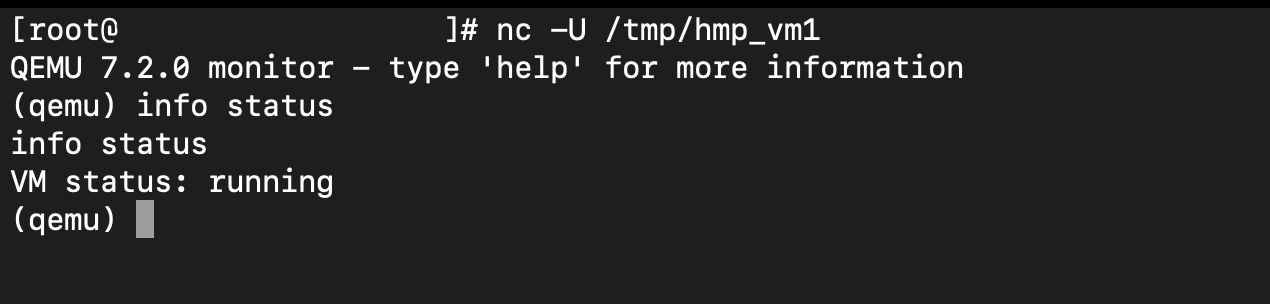
\includegraphics[width=\textwidth]{Images/QEMU Monitor.png}
    \captionof{figure}{QEMU Monitor}
    \label{fig}
\end{center}

Both VNC and QEMU Monitor provide essential methods for interacting with VMs, catering to different needs—from graphical user interaction to in-depth configuration and management.

%% Testing Procedures
\section{Testing Procedures}

%% Life Cycle Testing
\subsection{Life Cycle Testing}
Life cycle testing is a crucial step in validating the stability and reliability of a virtual machine (VM). This test involves performing a series of operations on the VM, such as starting, rebooting, resetting, stopping, and shutting down. Each operation tests a specific aspect of the VM's lifecycle management. \mynewline

For instance, the reboot process ensures that the VM can restart without data loss or corruption, while the shutdown operation tests the VM’s ability to terminate processes gracefully. The reset function is particularly important for checking if the VM can recover from an unresponsive state without requiring a full shutdown. \mynewline

By systematically executing these operations, we verify the VM’s robustness and its ability to handle various states of operation under different conditions. The results of these tests indicate whether the VM can consistently manage transitions between these states, which is essential for maintaining the overall health of the virtualization environment.

%% VNIC Hotplug/Unplug
\subsection{VNIC Hotplug/Unplug}
The VNIC (Virtual Network Interface Card) Hotplug/Unplug test evaluates the VM's capability to dynamically add and remove network interfaces without requiring a reboot. In this test, some VNICs are sequentially added and removed from the VM, and the system’s behavior is closely monitored. \mynewline

This test is critical for scenarios where network scalability and flexibility are required. The key focus is on ensuring that the VM can recognize new VNICs and reconfigure itself accordingly, as well as correctly release resources when VNICs are removed. This involves not only the successful attachment and detachment of the VNICs but also verifying that the network performance remains stable throughout the process.

%% VFIO-VNIC Hotplug/Unplug
\subsection{VFIO-VNIC Hotplug/Unplug}
The VFIO-VNIC Hotplug/Unplug test builds on the standard VNIC test by introducing Virtual Functions (VFs) through the VFIO (Virtual Function I/O) framework. VFs are essentially lightweight versions of physical network interfaces that provide dedicated resources for high-performance network operations. In this test, VFs are created from a physical VNIC and then hotplugged and unplugged in varying quantities.\mynewline

The objective is to assess whether the VM can efficiently handle these operations and make use of the VFs without compromising performance or stability. The test also examines how the VM manages the allocation and deallocation of hardware resources associated with VFs. Successful execution of this test demonstrates the VM’s ability to support advanced networking features, which is crucial for applications requiring high throughput and low latency.

%% VDisk Hotplug/Unplug
\subsection{VDisk Hotplug/Unplug}
The vDisk Hotplug/Unplug test is designed to assess the system's ability to dynamically manage storage resources. During this test, multiple virtual disks (vDisk) are added and removed from the running virtual machine (VM) to observe how well the system adapts to these changes without requiring a reboot or shutdown.\mynewline

The process begins by attaching one or more vDisks to the VM and verifying that the guest OS recognizes the newly added storage devices. This involves checking whether the disks are correctly identified in the OS, ensuring they can be mounted, partitioned, and used for file operations without errors. Afterward, these disks are detached, and the system's response is monitored to confirm that the detachment is clean, with no lingering references or errors in the OS logs.

%% Memory Hotplug/Unplug
\subsection{Memory Hotplug/Unplug}
The Memory Hotplug/Unplug test focuses on evaluating the VM's ability to handle changes in memory allocation during runtime. In this test, additional memory is dynamically added to a VM to see if the guest OS can recognize and utilize the extra RAM without requiring a restart. This is followed by the removal of the added memory to check whether the system can gracefully release the memory back to the host without any stability issues.\mynewline

The test procedure includes monitoring system logs and performance metrics to ensure that memory management functions correctly during the hotplug and unplug processes. This testing is vital in scenarios where workloads vary and demand flexible memory management, such as in virtualized data centers.

%% VCPU Hotplug/Unplug
\subsection{VCPU Hotplug/Unplug}
The vCPU Hotplug/Unplug test is performed to verify the system's capability to dynamically adjust processing power by adding or removing virtual CPUs (vCPUs) to the VM while it is running. The test starts by incrementally adding vCPUs to the VM and verifying that the guest OS detects and utilizes the additional processing resources. This involves running CPU-intensive tasks to observe if the additional vCPUs contribute to improved performance. Subsequently, vCPUs are removed, and the system's ability to redistribute the remaining processing workload without causing instability or performance degradation is assessed.\mynewline

The process is carefully monitored for any signs of errors or inefficiencies in CPU scheduling and task handling. This test is particularly important in environments where computing demands fluctuate, necessitating a scalable processing capability.

%% Kdump Check
\subsection{Kdump Check}
Kdump is a kernel crash dumping mechanism that captures system state information during a crash, aiding in post-crash analysis. To verify Kdump's functionality, the following steps were performed:

\begin{itemize}
    \item Enable SysRq Trigger using: \texttt{sysctl -w kernel.sysrq=1};
    \item A Kernel crash was manually induced using: \texttt{echo c > /proc/sysrq-trigger};
    \item After rebooting, the presence of crash logs in \texttt{/var/crash} or \texttt{/var/oled/crash} was checked to confirm Kdump's functionality.
\end{itemize}

This process ensures that Kdump is correctly capturing crash data, essential for system diagnostics.

%% Big VM 500G-1T Boot Test
\subsection{Big VM 500G-1T Boot Test}
In the Big VM 500G-1T Boot Test, the VM's memory allocation is significantly increased, first to 500GB and then to 1TB, to test its ability to boot with such large memory configurations. This test is critical for verifying the scalability of the VM in handling large workloads that require substantial memory resources.\mynewline

The boot process is carefully monitored to ensure that the VM can initialize and manage the expanded memory without encountering errors or significant delays. Successfully passing this test demonstrates the VM’s capability to support high-memory environments, which is essential for enterprise-level applications and large-scale data processing tasks.

\section{Conclusion}
This chapter has detailed the primary tasks of the internship, focusing on QEMU and Libvirt tests. It covered the setup of environments, installation procedures, and the creation of virtual machines using both QEMU and Libvirt. These processes form the foundation for testing and validating virtualized environments, ensuring that the systems perform as expected across different configurations.